\documentclass[10pt]{article}
\usepackage{amsmath}
\usepackage{amsfonts}
\usepackage{amssymb}
\usepackage{amsthm}
\usepackage{graphicx}   %Include graphics
\usepackage{float}      %Used to force graphics to stay where I want them to stay
\usepackage{mathrsfs}   %for Fourier transform 'F' symbol \mathscr{F}
\usepackage{hyperref}   %For hyperlinks in the PDF
\usepackage{enumitem}   %so we can have nonIndented lists and enumerations
\usepackage{caption}
\usepackage{subcaption}


\pdfpagewidth 8.5in
\pdfpageheight 11in
\setlength{\oddsidemargin}{-.35in}
\setlength{\textwidth}{7.32in}
\setlength{\topmargin}{-.6in}
\setlength{\textheight}{9.4in}

%%%%%%%%%%%%%%%%%%%%%%%%%%%%%%%%%%%%%%%%%%%%%%%%%%%%%%%%%%

%matrix macro
\newcommand{\mat}[2][ccccccccccccccc]{\left [\!\!\begin{array}{#1} #2\\ \end{array} \!\!\right]}
\newcommand{\determ}[2][ccccccccccccccc]{\left| \begin{array}{#1} #2\\ \end{array} \right| \vspace{.5em}}

%permutation
\newcommand{\perm}[2][ccccccccccccccc]{\left (\begin{array}{#1} #2\\ \end{array} \right) \vspace{.5em}}

%piecewise function
%  example:
%     $$H_i(K, K_0)\iso\piece{ \trivial & \text{if $i=0$} \\ \bbz/2\bbz &\text{if $i=1$} \\ \trivial & \text{if $i\ge2$}}$
%
\newcommand{\piece}[2][cll]{\left \{\begin{array}{#1} #2\\ \end{array} \right. }

%system of equations
\newcommand{\sys}[2][lll]{\left \{\begin{array}{#1}#2 \\ \end{array} \right. }

%integral
\newcommand{\dint}{\displaystyle\int}

%sum
\newcommand{\dsum}[3]{
           \displaystyle\sum_{#1}^{#2} #3 }

%sum start i=0
\newcommand{\dsumiz}[2]{
           \displaystyle\sum_{i=0}^{#1} #2}

%sum start i=1
\newcommand{\dsumio}[3]{
           \displaystyle\sum_{i=1}^{#2} #3 }


%sets {b,...,e} and sets with conditions {x | x is an integer}
\newcommand{\set}[2]{  \left\{#1,\ldots,#2\right\} }
\newcommand{\dset}[2]{  \left\{#1\; :\;\;#2\right\} }
\newcommand{\plist}[2]{  \left(#1,\ldots,#2\right) }

\newcommand{\iso}{\cong}
\newcommand{\abs}[1]{ \left|#1\right|}
\newcommand{\pdfrac}[2]{\!\left(\dfrac{#1}{#2}\right)\! }
\newcommand{\pfrac}[2]{\!\left(\frac{#1}{#2}\right)\! }

\newcommand{\libzptrl}[2]{\dfrac{\partial #1}{\partial #2} }
\newcommand{\plibzptrl}[2]{\left(\dfrac{\partial #1}{\partial #2}\right) }
\newcommand{\libz}[2]{\dfrac{d #1}{d #2} }
\newcommand{\plibz}[2]{\left(\dfrac{d #1}{d #2}\right) }
\newcommand{\eval}[2]{\bigg|_{#1}^{#2}}
\newcommand{\transpose}[1]{{#1}\!^T\!}

\newcommand{\mean}{\mbox{E}}
\newcommand{\var}{\mbox{V}}
\newcommand{\cor}{\mbox{Cor}}

\newcommand{\inn}{^{\mbox{inn}}}
\newcommand{\out}{^{\mbox{out}}}
\newcommand{\innL}{^{\mbox{innL}}}
\newcommand{\innR}{^{\mbox{innR}}}
\newcommand{\outL}{^{\mbox{outL}}}
\newcommand{\outR}{^{\mbox{outR}}}
\newcommand{\iloe}{^{\mbox{iloe}}}
\newcommand{\olie}{^{\mbox{olie}}}
\newcommand{\iloeL}{^{\mbox{iloeL}}}
\newcommand{\iloeR}{^{\mbox{iloeR}}}
\newcommand{\olieL}{^{\mbox{olieL}}}
\newcommand{\olieR}{^{\mbox{olieR}}}
\newcommand{\m}{^{{\mbox{m}}}}
\newcommand{\mL}{^{{\mbox{mL}}}}
\newcommand{\mR}{^{{\mbox{mR}}}}
\newcommand{\comp}{^{{\mbox{c}}}}
\newcommand{\inv}{^{-1}}
\newcommand{\pprime}{^{\prime\prime}}
\newcommand{\erf}{\mbox{Erf}\,}
\newcommand{\Span}{\mbox{span}}

\newcommand{\trivial}{\{0\}}						%trivial group (abelian) {0}
\newcommand{\cbrace}[1]{\left\{#1\right\}}				%curly-braces {parameter}
\newcommand{\gen}[1]{\left\langle#1\right\rangle}
\newcommand{\norm}[1]{\left|\left|#1\right|\right|}
\newcommand{\dsup}[1]{displaystyle{\sup_{#1}}}
\newcommand{\range}{\mathrm{range}\;}
\newcommand{\trace}{\mathrm{trace}\;}
\newcommand{\lcm}{\mathrm{lcm}\;}
\newcommand{\clos}{\mathrm{clos\!}\;}
\newcommand{\supnorm}[1]{\norm{#1}_\infty}
\newcommand{\clin}{\mathrm{clin\!}\;}
\newcommand{\lin}{\mathrm{lin\!}\;}

\newcommand{\tuple }[2]{\left(#1, #2\right)}
\newcommand{\paren}[1]{\!\left(#1\right)\!}
\newcommand{\bracket}[1]{\left[#1\right]}
\newcommand{\inprod}[2]{\left\langle#1,#2\right\rangle}

\renewcommand\Re{\operatorname{Re}}
\renewcommand\Im{\operatorname{Im}}

\newcommand{\degree}{\ensuremath{^\circ}}
\newcommand{\overbar}[1]{\mkern 1.5mu\overline{\mkern-1.5mu#1\mkern-1.5mu}\mkern 1.5mu}
\newcommand{\Lim}[1]{\raisebox{0.5ex}{\scalebox{0.8}{$\displaystyle \lim_{#1}\;$}}}


%%%%%%%Boxes%%%%%%%%%%%%%%
\newcommand{\fpbox}[2]{
       \fbox{\parbox{#1}{#2}}
}
\newcommand{\cfbox}[1]{
\begin{center}
       \fbox{#1}
\end{center}
}
%%%%%%%%%%%%%%%%%%%%%%%%%%


%black board font
\newcommand{\bbc}{\mathbb{C}}
\newcommand{\bbd}{\mathbb{D}}
\newcommand{\bbf}{\mathbb{F}}
\newcommand{\bbn}{\mathbb{N}}
\newcommand{\bbz}{\mathbb{Z}}
\newcommand{\bbq}{\mathbb{Q}}
\newcommand{\bbr}{\mathbb{R}}
\newcommand{\bbt}{\mathbb{T}}
\newcommand{\bbx}{\mathbb{X}}
\newcommand{\bbu}{\mathbb{U}}

%script font
\newcommand{\sca}{\mathcal{A}}
\newcommand{\scb}{\mathcal{B}}
\newcommand{\scs}{\mathcal{S}}
\newcommand{\scl}{\mathcal{L}}
\newcommand{\scu}{\mathcal{U}}
\newcommand{\scm}{\mathcal{M}}
\newcommand{\sck}{\mathcal{K}}
\newcommand{\scf}{\mathcal{F}}
\newcommand{\sch}{\mathcal{H}}

\newcommand{\KL}{\mathcal{KL}}

 \renewcommand{\i}{\mathrm{i}}

\newcommand{\tinyspace}{5em }
\newcommand{\mediumspace}{10em }
\newcommand{\largespace}{10em }
\newcommand{\largerspace}{20em }
\newcommand{\hugespace}{40em }
\newcommand{\seperator}{\underline{\hspace{45em}}}

%%%%%%%%%%%%%%%%%%%%%%%%%%%%%%%%%%%%%%%%%%%%%%%%%%%%%%%%%%

%stretch rows of a table
\renewcommand*\arraystretch{1.10}

\pagestyle{plain}
\begin{document}

    \title{AMS 232 Nonlinear Optimization Hw \#2}
    \author{}
    \date{\today}
    \maketitle

The following system describes the dynamics of an inverted pendulum where the moment of inertia of the pendulum and the friction between the pendulum and the cart are negligible.  Defining $x_1$ as cart position, $x_2$ as cart velocity, $x_3$ as the angle between the pendulum and the positive vertical direction $x_4$ as the angular velocity, and $u$ is the force applied to the cart, we have the dynamics of the system as
      \begin{align}
         x_1 &= x_2 \\
         x_2 &= \dfrac{mLx_4^2\sin x_3-mg\sin x_3\cos x_3}{M + m\sin^2x_3} + \dfrac{u}{M+m\sin^2x_3} \\
         x_3 &= x_4 \\
         x_4 &= \dfrac{g(m+M)\sin x_3 - Lmx_4^2\sin x_3}{LM+Lm\sin^2x_3} - \dfrac{u\cos x_3}{LM+Lm\sin^2x_3}
      \end{align}
      Where $M, m, L$ are the mass of the cart, mass of the pendulum and length to the center of mass of the pendulum.

%Problem Set
\begin{enumerate}[leftmargin=*]
   \item Linearize the inverted pendulum system about the equilibrium point $x^*=\mat{0&0&0&0}^T$ when given the input $u^*=0$.  We linearize about the equilibrium $x^*=0,u^*=0$ by $\dot x = Ax+Bu$ where $A=\libzptrl{f}{x}\eval{x^*,u^*}{}$ is a $4\times4$ real matrix and $B=\libzptrl{f}{u}\eval{x^*,u^*}{}$ is a $4\times1$ vector.  As $f:\bbr^4\longrightarrow\bbr^4$ and $u\in\bbr$ we have that
       \begin{align*}
            A &= \libzptrl{f}{x}\eval{x^*,u^*}{}
               = {\mat{ \libzptrl{f_1}{x_1}&\cdots&\libzptrl{f_1}{x_4} \\
                       \vdots & &\vdots \\
                       \libzptrl{f_4}{x_1}&\cdots&\libzptrl{f_4}{x_4} }}_{|x^*,u^*}
               = \mat{0 & 1 & 0 & 0 \\
                      0 & 0 & -\frac{gm}{M} & 0 \\
                      0 & 0 & 0 & 1 \\
                      0 & 0 & \frac{g(m+M)}{LM} & 0} \\\\
            B &=  \libzptrl{f}{u}\eval{x^*,u^*}{} = {\mat{\libzptrl{f_1}{u} \\ \vdots \\ \libzptrl{f_4}{u}}}_{|x^*,u^*}
              = \mat{0 \\ \frac{1}{M} \\ 0 \\ -\frac{1}{LM}}
       \end{align*}
\qed\\
   Consider the infinite horizon optimal control problem:
   \begin{equation*}
        \begin{aligned}
            & {\text{minimize}} & &J[x(\cdot),u(\cdot)]=\frac{1}{2}\int_0^\infty x^TQx+u^TRu\,dt \\
            & \text{subject to} & &\dot x = Ax+Bu \\
                                & & & x(t_0)=x^0\in\bbr^4
        \end{aligned}
      \end{equation*}
   Where $R=1$, $Q$ is a diagonal matrix with the main diagonal as $\mat{1 & 0 & 1 & 0}$.  Note, for an infinite horizon LQR problem to be well defined, we need $(A,B)$ controllable and $(A,Q^{1/2})$ to be observable, which is the case (Chen, Linear Control Text).  Since $A, B, Q, R$ are all time invariant, and that we are minimizing an infinite horizon problem, we have that the optimal feedback controller for this problem is given by the constant gain $K=-R\inv B^TP$ (so $u^*=Kx$) where $P$ is the solution to the algebraic Riccati equation
   \begin{align*}
        PA+A^TP-P(BR\inv B^T)P+Q=0
   \end{align*}
   See M. Ross' text (A Primer on Pontryagin's Principle in Optimal Control), section 3.4 for a full reference.

   \item Here we numerically solve the algebraic Riccati equation.  To solve the algebraic Riccati equation, we implemented the method presented in the paper ``A Schur Method for Solving Algebraic Riccati Equations'' by Alan J. Laub.  See Theorem 5, part 1 of the paper.  Attached is some code to solve an algebraic Riccati equation; use it to validate the examples presented in the paper.  With $A,B,R, Q$ given after problem 1, the solution $P$ to $PA+A^TP-P(BR\inv B^T)P+Q=0$ is
       \begin{align*}
       P=\mat{
            1.49043264127365 &	1.11069472908698 &	2.73480164461872 &	0.483208418726095 \\
            1.11069472908698 &	1.37635428641379 &	3.59282921982252 &	0.636471182115187 \\
            2.73480164461872 &	3.59282921982250 &	23.5303741786798 &	3.73957001770460 \\
            0.483208418726094 &	0.636471182115184 &	3.73957001770461 &	0.601161601327363
            }
       \end{align*}

    \item Substituting our feedback control $u^*=Kx=-R\inv B^TPx$ into the dynamics $\dot x = Ax+Bu$ we have $\dot x = (A-BR\inv B^TP)x$, which is a stable system, as every eigenvalue of the matrix $A-BR\inv B^TP$ has negative real part.  Therefore as $t\longrightarrow\infty$, $x\longrightarrow0$.  The following figures are simulations of the closed loop performance of the linearized inverted pendulum, obtained by running the MatLab code attached at the end of this document.

         \begin{figure}[H]
            \centering
            \begin{minipage}{.5\textwidth}
              \centering
              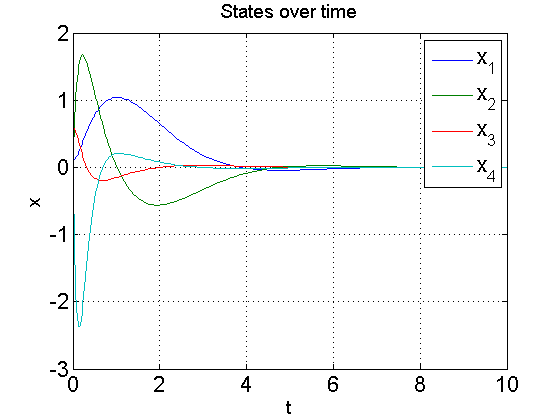
\includegraphics[width=1.\linewidth]{s1state.png}
              \captionsetup{width=0.8\textwidth}
              \captionof{figure}{States over time given the initial condition $x_0=\mat{0.1 & 0.1 & 0.6 & 0.1}$.}
            \end{minipage}%
            \begin{minipage}{.5\textwidth}
              \centering
              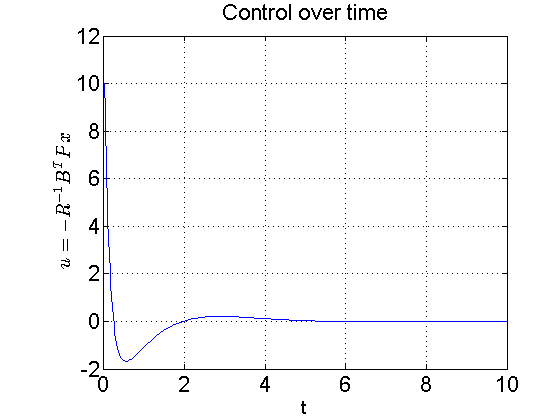
\includegraphics[width=1.\linewidth]{s1ctrl.png}
              \captionof{figure}{Control $u=Kx$ over time given the initial condition $x_0=\mat{0.1 & 0.1 & 0.6 & 0.1}$.}
            \end{minipage}
         \end{figure}


         \begin{figure}[H]
            \centering
            \begin{minipage}{.5\textwidth}
              \centering
              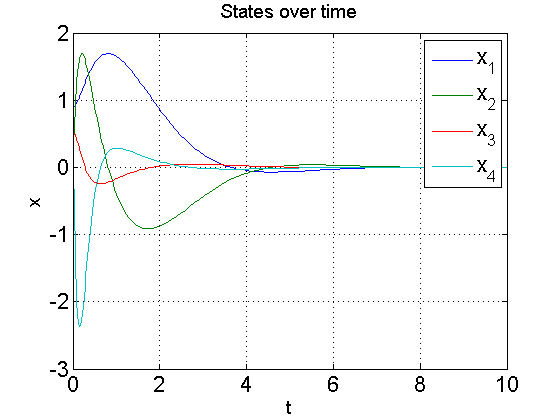
\includegraphics[width=1.\linewidth]{s2state.png}
              \captionsetup{width=0.8\textwidth}
              \captionof{figure}{States over time given the initial condition $x_0=\mat{0.9 & 0 & 0.5 & 0.9}$.}
            \end{minipage}%
            \begin{minipage}{.5\textwidth}
              \centering
              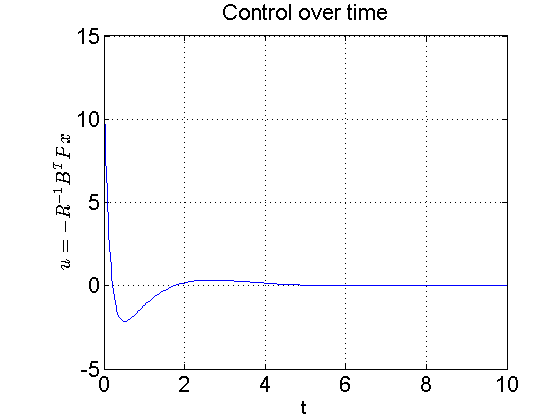
\includegraphics[width=1.\linewidth]{s2ctrl.png}
              \captionof{figure}{Control $u=Kx$ over time given the initial condition $x_0=\mat{0.9 & 0 & 0.5 & 0.9}$.}
            \end{minipage}
         \end{figure}


         \begin{figure}[H]
            \centering
            \begin{minipage}{.5\textwidth}
              \centering
              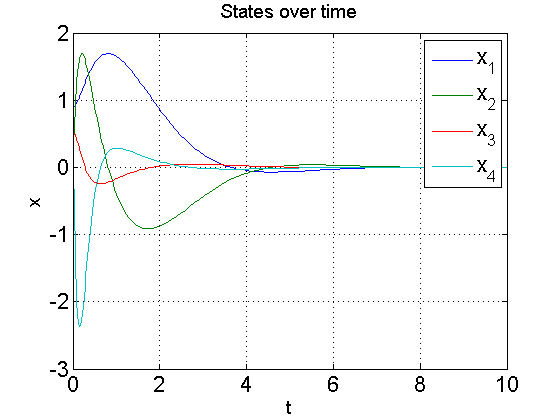
\includegraphics[width=1.\linewidth]{s2state.png}
              \captionsetup{width=0.8\textwidth}
              \captionof{figure}{States over time given the initial condition $x_0=\mat{0 & 0.6 & 0 & 0.9}$.}
            \end{minipage}%
            \begin{minipage}{.5\textwidth}
              \centering
              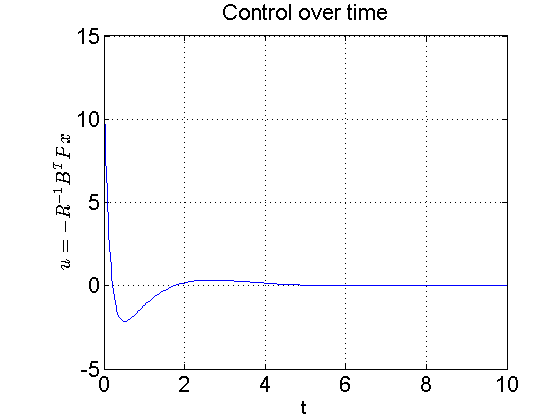
\includegraphics[width=1.\linewidth]{s2ctrl.png}
              \captionof{figure}{Control $u=Kx$ over time given the initial condition $x_0=\mat{0.1 & 0.1 & 0.6 & 0.1}$.}
            \end{minipage}
         \end{figure}

    \item Lastly, we analyze the effect of the closed loop performance to the inverted pendulum when varying $R$.  As $R$ is increased the time to reach the equilibrium increases.
        
        \begin{figure}[H]
            \centering
            \begin{minipage}{.5\textwidth}
              \centering
              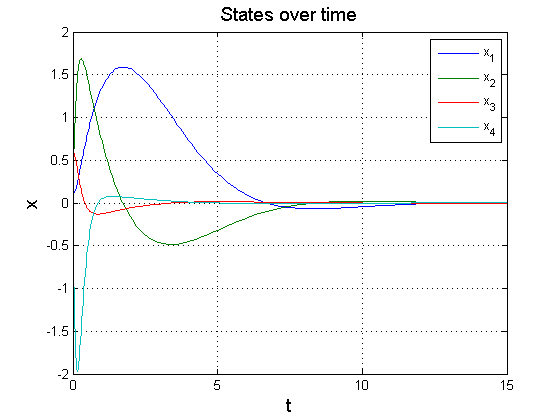
\includegraphics[width=1.\linewidth]{Ris10.png}
              \captionsetup{width=0.8\textwidth}
              \captionof{figure}{With $R=10$, we see the states settle to the equilibrium around 11 seconds.}
            \end{minipage}%
            \begin{minipage}{.5\textwidth}
              \centering
              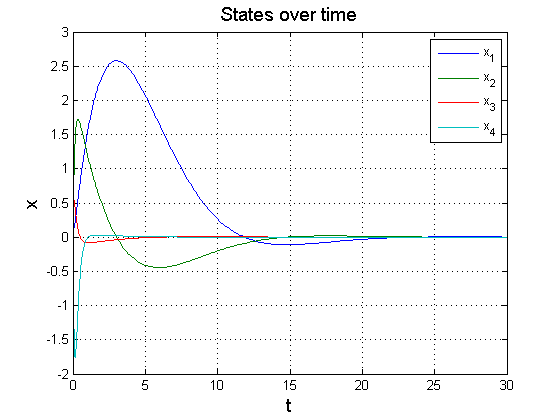
\includegraphics[width=1.\linewidth]{Ris100.png}
              \captionof{figure}{With $R=100$, we see the states settle to the equilibrium around 23 seconds.}
            \end{minipage}
         \end{figure}
         
\end{enumerate}


\newpage
\subsection*{Matlab Code}{

    \subsection*{hw2.m}{
        \begingroup
        \fontsize{7pt}{7pt}
        \begin{verbatim}
%{
    Infinite Horizon LQR problem, HW #2 from AMS 232
%}
clear all;
close all;


%Simulation Parameters of the Inverted Pendulum
g = 9.8;    %m/s^2, downward is positive
m = 0.2;    %kg
M = 0.5;    %kg
L = 0.3;    %m

%A and B are the Linearized (Control) system
A = [0  1         0         0;
     0  0     -(g*m)/M      0;
     0  0         0         1;
     0  0  (g*(m+M))/(L*M)  0 ];
B = [0; 1/M; 0; -1/(L*M)];

%LQR simulation parameters
R = 1;
Q = diag([1 0 1 0]);

%The problem is an infinite horizon problem, so we set the final time to be large
t0=0;
tf=5;

x0 = [.1;.1;.6;.1];

%Example initial conditions
% ex1:  [.1;.1;.6;.1]
% ex2:  [.9;0;.5;.9]
% ex3:  [0;.6;0;.9]
% ex4:  [10;10;10;10] %the control for the linearized system fails for this large initCond

%Note, you should Check the Controllability of (A,B)
%Note, you should Check Observability of (A, sqrt(Q))
%If both tests are passed, then the problem is well defined

%Get P by solving the Continuous Time Algebraic Riccati Equation
P = solveContTimeAlgRiccati(A, B, Q, R);

% % We can check that indeed the CT Alg Riccati Equation is solved, just uncomment out the
% following two lines.
% checkResult = A'*P + P*A - P*( B*inv(R)*B' )*P + Q;
% norm(Result)

%The gain
K = -R*B'*P;

%Now we solve for the state x as \dot x = (A-B*inv(R)*B'*P)*x  the system is stable as
%all eigenvalues of (A-B*inv(R)*B'*P) have negative real part
linearSystem = @(t,x) (A-B*inv(R)*B'*P)*x;

%Just for fun, we get solve for x in the nonlinear system, passing-in the gain as the
%control.  For initial conditions near the equalibrium, both will result with the same
%state trajectories, but for large initial conditions, the linearization fails.
nonLinSystem =  @(t,x) ...
          [x(2);
          (m*L*x(4)^2*sin(x(3)) - m*g*sin(x(3)).*cos(x(3)))./(M+m*sin(x(3)).^2) + (K*x)./(M+m*sin(x(3)).^2);
          x(4);
          ((m+M)*g*sin(x(3)) - L*m*x(4)^2*sin(x(3)).*cos(x(3)))./(L*M + L*m*sin(x(3)).^2) - (K*x*cos(x(3)))./(L*M + L*m*sin(x(3)).^2)];

[tLin, xLinOpt] = ode45( linearSystem, [t0 tf], x0);
[tNonLin, xNonLin] = ode45( nonLinSystem, [t0 tf], x0);

%The optimal control is u=-R*B'*P*x where s is the solution
%to \dot x = (A-B*inv(R)*B'*P)*x
uOpt = K*xLinOpt';


%%%% Pretty Plot code %%%%
figure;
    plot(tLin, xLinOpt);
    title('States over time','fontSize',14);
    xlabel('t','fontSize',14);
    ylabel('x','fontSize',14);
    legend('x_1', 'x_2', 'x_3', 'x_4');
    grid on;

figure;
    plot(tLin, uOpt);
    title('Control over time');
    xlabel('t','fontSize',14);
    ylabel('$u=-R^{-1}B^TPx$','Interpreter','LaTex','fontSize',14);
    grid on;

%Plotting the state of the nonLinear system given the linearized control.
figure;
    plot(tNonLin, xNonLin);
    title('NonLinear System under the control u=Kx');
    grid on;
%
%   end hw2.m
%
        \end{verbatim}
        \endgroup
    }

    \subsection*{solveContTimeAlgRiccati.m}{
        \begingroup
        \fontsize{7pt}{7pt}
        \begin{verbatim}
%{
    This function solves the continuous time algebraic Riccati Equation, given
        A nxn
        B nx1
        Q nxn
        R 1x1
    We use the procedure from the paper ''A Schure Method for Solving Algebraic Riccati
    Equations'' by Alan J. Laub--See section II, theorem 5
%}
function [ P ] = solveContTimeAlgRiccati( A, B, Q, R )

    %A is a square matrix, so grab the number of rows n.
    [n,~] = size(A);

    %The Hamiltonian system  xDot      =  partial{H}/partial{lambda} and
    %                        lambdaDot = -partial{H}/partial{x}
    hamilSystem = [ A -(B*inv(R))*B' ; -Q -A'];

    %Perform a Schur Decomposition, and then reorder it so all of the negative eigenvalues
    %come first
    [U, T] = schur(hamilSystem);
    [US, TS] = ordschur(U,T,'lhp');

    %U11 and U12 match part (1) of Theorem 5
    U11 = US(1:n, 1:n);
    U21 = US((n+1):(2*n), 1:n);

    %result from part(1) of Theorem 5
    P = U21*inv(U11);

end

%
% end solveContTimeAlgRiccati.m
%
        \end{verbatim}
        \endgroup
    }
}

\end{document} 